%%=============================================================================
%% Methodologie
%%=============================================================================

\chapter{Resultaat van de Enquête}
\label{ch:resultaten_vragen}

In totaal vulden in de periode tussen 8 april en 7 mei 404 studenten, verspreid over de Hogeschool Gent in België en de Haagse Hogeschool in Nederland, de enquête in. Het nam de student gemiddeld 7 minuten en 52 seconden om de enquête in te vullen.

\begin{figure}
	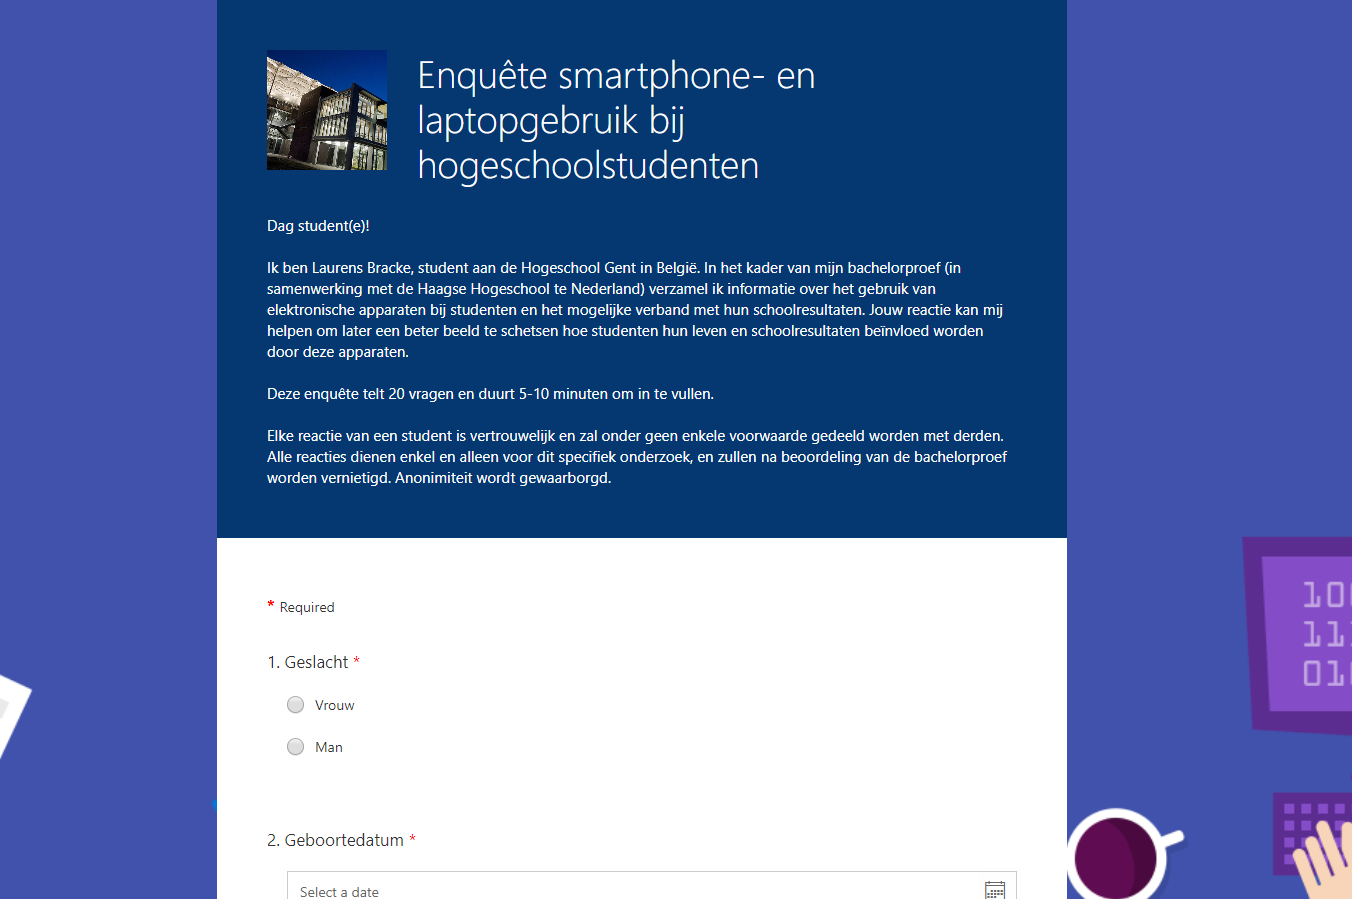
\includegraphics[width=\textwidth]
	{img/vragen-enquete.png}
	\caption{Vragen enquete voor studenten Haagse Hogeschool en HoGent }
	\label{fig:vragen-enquete}
\end{figure}

In figuur \ref{fig:vragen-enquete} vindt u een screenshot terug van de online vragenlijst over hun gebruik van smartphones, laptops en hun studieresultaten. 

De vragen (met correcte antwoorden) kan u terugvinden in bijlage \ref{ch:vragenlijst}.

De resultaten van deze test kan u terugvinden via volgende weblink (in Excel-formaat): \url{https://1drv.ms/f/s!AnudQT05fzZSlx83i8B1_PG0OKxa} 

Door middel van het gebruik van een steekproefcalculator (bijvoorbeeld \url{nl.checkmarket.com/steekproefcalculator}) en het cijfermateriaal uit de literatuurstudie kunnen we vaststellen dat het aantal resultaten dat we nodig hadden voor significante resultaten te bekomen dit onderzoek tekort schiet. Indien we zowel in Nederland als in België nog 100 extra studenten konden bereiken in deze periode, konden we mogelijks spreken van een significant onderzoek dat de volledige populatie benadert met een betrouwbaarheidsinterval van 95 procent. De Vlaamse resultaten mogen wel significant genoemd worden als we rekenen met een betrouwbaarheidsinterval van 90 procent. Onze resultaten zijn wel nog steeds een goede indicatie van de onderzochte groep. Volgens vernoemde site kunnen we stellend dat de bekomen resultaten moeten bekeken worden met een foutmarge van 7,51 procent voor Nederland en een foutmarge van 6,16 voor België. We gaan hier uit dat van alle verzonden invitaties via Facebook, e-mail of mondelinge communicatie 15 à 20 procent geantwoord hebben (Checkmarket.com geeft aan de kans dat iemand een antwoord geeft op een online enquête ongeveer 20 procent is, hoewel ze zelf aangeven dat dit een zeer positieve inschatting is).

Om deze resultaten te onderzoeken, zullen we een tabel maken die bestaat uit 3 kolommen: de eerste kolom vat de resultaten van alle 404 antwoorden samen, de tweede kolom is een samenvatting van de resultaten van studenten die minder of evenveel tijd spenderen achter hun smartphone of laptop per dag dan het gemiddelde waar de derde kolom die studenten zal groeperen die qua gespendeerde tijd achter hun devices over het gemiddelde scoren. In tabel \ref{} ziet u hiervan de uitkomst.

Aan de hand van deze tabel overlopen we hieronder alle onderzoeksvragen die we bij dit onderzoek hebben gesteld en bekijken we de resultaten / meningen van de student.

\section{VRAAG 1: Heeft het gebruik van smartphones en laptops tijdens de lessen mogelijks een invloed op de slaagcijfers en kennis van de student?}
\label{sec:hoofdvraag}


\section{VRAAG 2: Heeft geslacht, relatiestatus of leeftijd van de student een invloed op de aantrekkingskracht die deze devices hebben op de student?}
\label{sec:geslacht-leeftijd}


\section{VRAAG 3: Is er een verschil in omgang met devices tussen Nederlandse en Vlaamse studenten?}
\label{sec:vlaanderen-nederland}

\begin{figure}
	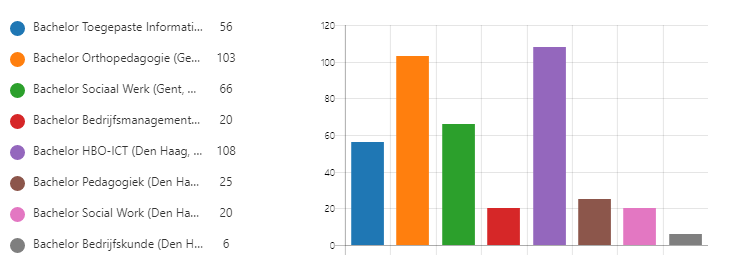
\includegraphics[width=\textwidth]
	{img/verdeling-enquete-richting.png}
	\caption{Verdeling van de studenten die geantwoord hebben op de enquête op basis van hun studierichting (totaal: 404)}
	\label{fig:verdeling-enquete-richting}
\end{figure}

\section{VRAAG 4: Wat denken studenten zelf over de invloed van smartphones op hun resultaten?}
\label{sec:invloed-resultaten}


\section{VRAAG 5: Is er een verschil in gebruik van smartphones en in resultaten tussen studenten uit een sociale richting en studenten uit een richting die IT-gerelateerd is?}
\label{sec:sociale-it-richting}




\begin{figure}
	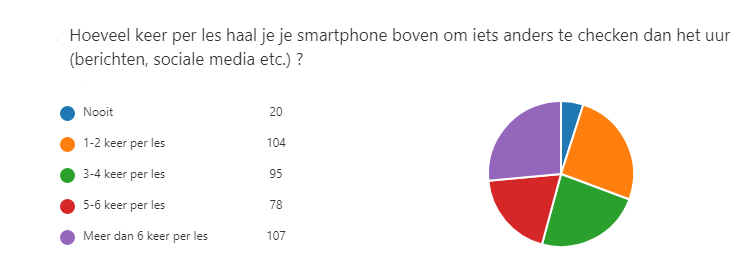
\includegraphics[width=\textwidth]
	{img/smartphone-social.png}
	\caption{Aantal keer dat studenten hun smartphone checken per les volgen de enquête (totaal: 404)}
	\label{fig:smartphone-social}
\end{figure}

\begin{figure}
	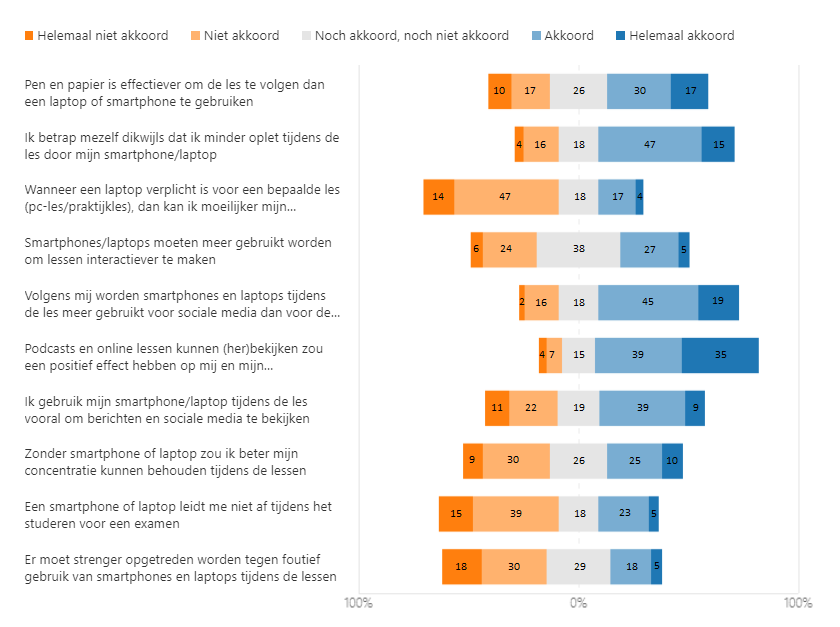
\includegraphics[width=\textwidth]
	{img/stellingen.png}
	\caption{Antwoorden van studenten op 10 stellingen over hun devices en de lessen (percentages afgerond naar gehele getallen)}
	\label{fig:stellingen}
\end{figure}


